\section{Bases of General Relativity}

Let us first introduce a few basic concepts, which are the basic tools of General Relativity and that we will need in the remaining
of our project. Indeed the Einstein’s theory is based on radically
different concepts than the Newton’s ones and appeals to a certain number of mathematical object, such as tensors
which were not particularly widespread at the beginning of the twentieth century.

\subsection{Equivalence principle}

The fundamental principle of General Relativity is the Equivalence Principle. We
could say that this principle emerged in the late sixtieth century when Galileo
expressed experimentally that the acceleration of an object due to gravitation is
independent of its mass.
In other words, the equivalence principle stipulates that the inertial mass $m_{I}$, which defines the ability of an object
to move further a solicitation (a force), and the gravitational mass $m_{G}$, which is a coupling coefficient between the
same object and the gravitational field\footnote{It only depends on the object features.}, are strictly equals :
%
\begin{equation}
	m_{G} = m_{I} = m
\end{equation}
%
In classical physics, there is no reason to think that these two quantities are equal.
They can be only considered as coefficients corresponding to two different physical
phenomena. However, all the experiments made so far have shown that the Equivalence Principle is accurate within an
uncertainty of magnitude $10^{-11}$ \cite{schlamminger2008test}.
By establishing the General Relativity, Einstein held this principle as true, from which follows his famous thought experiment of the elevator :
taken an observer in a closed and accelerated elevator,
there is no possibility for him to know whether the acceleration that he feels is due to a gravitational effect or to the fact that his reference
frame is non-inertial. In other words, being at rest on the surface of the Earth is equivalent to being inside
a spaceship that is being accelerated by the amount of $g$.
As a consequence, taking a reference frame $\mathcal{R}$ in presence of a static and uniform gravitational field
$\textbf{g}$, we can define a \textit{free-falling} reference frame $\mathcal{R}'$ where the gravitational field is eradicated (Fig. \ref{equivalence_illus}) and where
the laws of inertia may be applied. Indeed, applying the second law of Newton to any point $M$ in $\mathcal{R}$, we have :
%
\begin{equation}
 m\mathbf{a} = m\tfrac{\mathrm{d}^2\mathbf{OM}}{\mathrm{d}t^2} = m \mathbf{g}
\end{equation}
%
while in $\mathcal{R}'$ we have
%
\begin{equation}
 m \mathbf{a'} = m\tfrac{\mathrm{d}^2\mathbf{O'M}}{\mathrm{d}t^2}
 = m \left( \tfrac{\mathrm{d}^2\mathbf{O'O}}{\mathrm{d}t^2} + \tfrac{\mathrm{d}^2\mathbf{OM}}{\mathrm{d}t^2}\right)
 = m\left(\mathbf{a} - \mathbf{g}\right) = \mathbf{0}
\end{equation}

%
since $\mathbf{O'O} = -\frac{1}{2}\mathbf{g}t^2$.
What we did for a static and uniform gravitational field can be generalized to a time and space-dependent field
$\mathbf{g}(t,\mathbf{x})$, which allows us to reformulate the Principle of Equivalence in these words :
%
\begin{figure}
\begin{center}
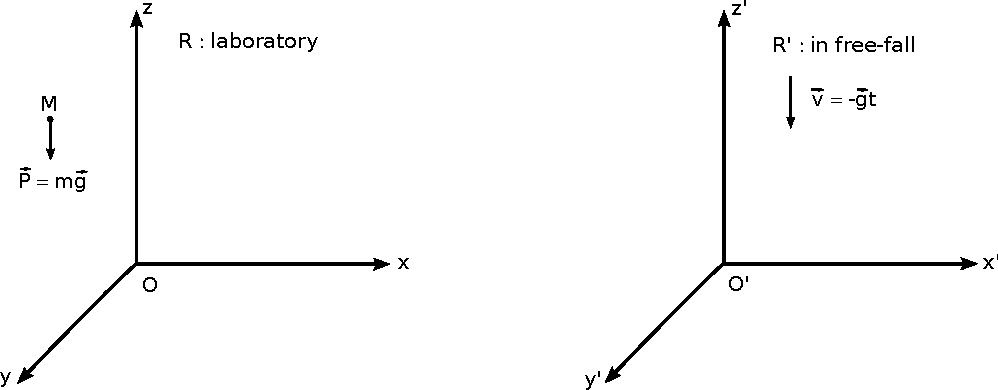
\includegraphics[width=\textwidth]{equivalence_principle.pdf}
\end{center}
\caption{We can eradicate the gravitational field by defining a free-falling frame.}
\label{equivalence_illus}
\end{figure}
\begin{center}
%
\textit{In every point $M$ of a gravitational field and at any time, it exists a reference frame of coordinate $\left\{\xi^\alpha\right\}$ locally
inertial in which the laws of Nature are
identical from those that exist in an inertial reference frame in absence of gravitation.}
\end{center}
%
The next step to cross is to make the analogy with differential geometry which states that near from any point
of a non-euclidean surface we can locally erect an euclidean coordinate system.
A straightforward example is that for someone on the Earth, looking around, Earth seems to be flat (Euclidean plan) but we know that it is spherical.
The case of interest for us would be rather Minkowskian coordinate system rather than Euclidean. Nevertheless, it can be generalized to this particular
case\footnote{The underlying mathematical structure is called a pseudo-Riemannian manifold.}.
This means that gravitation can be considered as a modification of space-time.
This principle involves several important facts that built the General Relativity theory:
%
\begin{itemize}
%
\item Gravitation is described by a metric theory. The effects of the gravitation depend only on the space-time metric coefficients as well as its derivatives.
\item The co-moving frame of an object in free-fall is a local frame of reference
in which the gravitation has been canceled out : there is always a local Minkowskian frame of reference for an isolated experience.
\item In a curved space-time, the world line (trajectory) of an inertial object is no longer a
straight line but the path that minimizes the distance between two points\footnote{It is a generalization of the straight line
for curved spaces where straight line is not necessary the shortest path between two points.}. Such a world line is called a geodesic.
%
\end{itemize}

\subsection{Geodesic equation}

Let consider a particle only under the influence of gravitational forces. According to the
Principle of Equivalence above, we can find a local inertial frame $\left\{\xi^\alpha\right\}$
where its equation of motion is a straight line in space-time :
%
\begin{equation}\label{geodesic_lif}
	\frac{\mathrm{d}^2\xi^\alpha}{\mathrm{d}\tau^2} = 0
\end{equation}
%
with d$\tau$ the proper time which expresses as :
%
\begin{equation}\label{proper_time1}
	\mathrm{d}\tau^2 = \eta_{\alpha\beta}\mathrm{d}\xi^\alpha\mathrm{d}\xi^\beta
\end{equation}
%
Now we take an other system of coordinates system $x^\mu$, which may be Cartesian coordinates
as spherical coordinates or whatever. The coordinates of the local inertial frame are 
consequently functions of $x^\mu$, that is $\xi^\alpha\left(x^\mu\right)$. So by basic
calculus, equation \eqref{geodesic_lif} becomes :
%
\begin{equation}
	\frac{\partial\xi^\alpha}{\partial x^\mu} \frac{\mathrm{d}^2x^\mu}{\mathrm{d}\tau^2}
	+ \frac{\partial^2\xi^\alpha}{\partial x^\mu \partial x^\nu}
	\frac{\mathrm{d}x^\mu}{\mathrm{d}\tau}\frac{\mathrm{d} x^\nu}{\mathrm{d}\tau} = 0
\end{equation}
%
Multiplying this by $\frac{\partial x^\lambda}{\partial \xi^\alpha}$ and using the rule :
%
\begin{equation}\label{product_rule}
	\frac{\partial\xi^\alpha}{\partial x^\mu}\frac{\partial x^\lambda}{\partial \xi^\alpha}
	= \delta^\lambda_\mu
\end{equation}
%
Finally gives us the geodesic equation :
%
\begin{equation}\label{formula:geodesic}
	\frac{\mathrm{d}^2x^\lambda}{\mathrm{d}\tau^2} + \Gamma^\lambda_{\mu\nu} 
	\frac{\mathrm{d}x^\mu}{\mathrm{d}\tau}\frac{\mathrm{d}x^\nu}{\mathrm{d}\tau} = 0
\end{equation}
%
where $\Gamma^\lambda_{\mu\nu}$ are called Christoffel symbols.
They are defined by :
%
\begin{equation}\label{affine_connection}
	\Gamma^\lambda_{\mu\nu} = \frac{\partial x^\lambda}{\partial \xi^\alpha}
	\frac{\partial^2\xi^\alpha}{\partial x^\mu \partial x^\nu}
\end{equation}
%
and we note that they are symmetric in the lower two indices.
The proper time $\mathrm{d}\tau$ may also be expressed in the new coordinate system :
%
\begin{equation}\label{proper_time2}
	\mathrm{d}\tau^2 = \eta_{\alpha\beta} \frac{\partial \xi^\alpha}{\partial x^\mu}
	\mathrm{d}x^\mu \frac{\partial \xi^\beta}{\partial x^\nu} \mathrm{d}x^\nu
\end{equation}
%
From here we introduce the metric tensor $g$ which the components are :
%
\begin{equation}\label{metric1}
	g_{\mu\nu} = \eta_{\alpha\beta} \frac{\partial \xi^\alpha}{\partial x^\mu}
	\frac{\partial \xi^\beta}{\partial x^\nu}
\end{equation}
%
and which are symmetric. As Minkowski metric in the case of special relativity,
it allows us to raise or to lower indices of a vector or a tensor by contraction :
%
\begin{equation}
 A_\mu = g_{\mu\nu} A^\nu \quad \mathrm{and} \quad A^\mu = g^{\mu\nu} A_\nu
\end{equation}
%
where $g^{\mu\nu}$ is the inverse of the metric tensor defined as :
%
\begin{equation}
	g_{\mu\lambda}g^{\lambda\nu} = \delta^\nu_\mu
\end{equation}
%
Finally, equation \eqref{proper_time2} may be expressed as :
%
\begin{equation}\label{invariant}
	\mathrm{d}\tau^2 = g_{\mu\nu}\mathrm{d}x^\mu\mathrm{d}x^\nu
\end{equation}
%
Geodesic equation is only available for massive particles. In fact, this cannot be use for
massless particles as photons because in this case, the right-hand side of
\eqref{proper_time1} vanishes. Nevertheless, calculus may be done by replacing $\tau$ in
\eqref{geodesic_lif} by any parameter, as $\sigma = \xi^0$ for example. In the remaining of the report,
we are going to restrict us only to massive particles.

\subsection{Christoffel symbols}

We have seen that Christoffel symbols and the metric tensor appeared naturally when we want to
express the equation of motion in an arbitrary coordinate system. Now we are going to see the
link between these two objects and thus the link between Christoffel symbols and the
structure of space-time, that is the metric.
For this aim, we have first to differenciate the metric tensor with respect to $x^\lambda$,
which gives :
%
\begin{equation}\label{equation_longue}
	\frac{\partial g_{\mu\nu}}{\partial x^\lambda} = 
	\eta_{\alpha\beta}\left(\frac{\partial^2 \xi^\alpha}{\partial x^\lambda\partial x^\mu}
	\frac{\partial \xi^\beta}{\partial x^\nu} +
	\frac{\partial \xi^\alpha}
	{\partial x^\mu}\frac{\partial^2\xi^\beta}{\partial x^\lambda \partial x^\nu}\right)
\end{equation}
%
To go further we need an extra relation which may be obtain by multiplying
\eqref{affine_connection} by $\frac{\partial \xi^\beta}{\partial x^\lambda}$ and by using
\eqref{product_rule}. That gives us :
%
\begin{equation}
	\frac{\partial^2 \xi^\alpha}{\partial x^\mu \partial x^\nu}
	= \Gamma^\lambda_{\mu\nu} \frac{\partial \xi^\alpha}{\partial x^\lambda}
\end{equation}
%
This relation allows to express \eqref{equation_longue} with Christoffel symbols :
%
\begin{equation}
	\frac{\partial g_{\mu\nu}}{\partial x^\lambda} = 
	\eta_{\alpha\beta}\left(\Gamma^\rho_{\lambda\mu}
	\frac{\partial\xi^\alpha}{\partial x^\rho}
	\frac{\partial \xi^\beta}{\partial x^\nu} + \Gamma^\rho_{\lambda\nu}
	\frac{\partial\xi^\alpha}{\partial x^\mu}
	\frac{\partial \xi^\beta}{\partial x^\rho}\right)
\end{equation}
%
Using \eqref{metric1}, we find :
%
\begin{equation}\label{equation_derive_metrique}
	\frac{\partial g_{\mu\nu}}{\partial x^\lambda} =
	\Gamma^\rho_{\lambda\mu}g_{\rho\nu} + \Gamma^\rho_{\lambda\nu}g_{\mu\rho}
\end{equation}
%
We recall that $\Gamma^\lambda_{\mu\nu}$ and $g_{\mu\nu}$ are symmetric under permutation of
$\mu$ and $\nu$. So by adding to \eqref{equation_derive_metrique} the same equation with
$\mu$ and $\lambda$ interchanged and by subtracting the same equation with $\nu$ and
$\lambda$ interchanged, we obtain :
%
\begin{equation}
\begin{aligned}
	\frac{\partial g_{\mu\nu}}{\partial x^\lambda}
	+ \frac{\partial g_{\lambda\nu}}{\partial x^\mu}
	- \frac{\partial g_{\mu\lambda}}{\partial x^\nu}
	& = g_{\sigma\nu} \Gamma^\sigma_{\lambda\mu} 
	+ g_{\sigma\mu} \Gamma^\sigma_{\lambda\nu} 
	+ g_{\sigma\nu} \Gamma^\sigma_{\mu\lambda} 
	+ g_{\sigma\lambda} \Gamma^\sigma_{\mu\nu} 
	- g_{\sigma\lambda} \Gamma^\sigma_{\nu\mu} 
	- g_{\sigma\mu} \Gamma^\sigma_{\nu\lambda} \\
	& = 2g_{\sigma\nu}\Gamma^\sigma_{\mu\lambda}
\end{aligned}
\end{equation}
%
Finally, we multiply each term by $g^{\nu\rho}$ an obtain the expected equation :
%
\begin{equation}\label{formula:christoffel}
	\Gamma^\sigma_{\mu\nu} =
	\frac{1}{2}g^{\sigma\lambda}\left\{\frac{\partial g_{\lambda\nu}}{\partial x^\mu}
	+ \frac{\partial g_{\mu\lambda}}{\partial x^\nu}
	- \frac{\partial g_{\mu\nu}}{\partial x^\lambda}\right\}
\end{equation}
%
Not only this relation gives the link between Christoffel symbols and geometrical structure
of space-time but also it provides a useful expression to compute these symbols. In fact, the
expression \eqref{affine_connection} leads to laborious calculus but adding properties
of symmetries of the symbols to relation \eqref{formula:christoffel}, these calculus are more easier as we will see later.
Moreover, we want to indicate that Christoffel symbols are not tensors. If it were the case,
since they are null in the good frame (a local inertial one), we might deduce by a change of frame
that they are null in all frames. By the way, in General Relativity we are no longer restricted to Lorentz transformation
in a change of frame but to any\footnote{That is the reason why \textit{General} Relativity.} diffeomorphism
$x^\mu \rightarrow {x'}^\nu$ and so components of a vector $\textbf{A}$ transform as :
%
\begin{equation}
 {A'}^\mu = \frac{\partial {x'}^\mu}{\partial x^\nu} A^\nu \quad \mathrm{and} \quad {A'}_\mu = \frac{\partial x^\nu}{\partial {x'}^\mu} A_\nu
\end{equation}

\subsection{Einstein field equations}

Before introducing the Einstein field equations that allows to determine the metric tensor $g_{\mu\nu}$ from the repartition of mass
and energy, we will need to introduce few more quantities that intervene in its expression.

\subsubsection{Ricci tensor}

The Ricci tensor, denoted $R_{\mu\nu}$, is a symmetric tensor and it is related to the Christoffel symbols by the
equation\footnote{To see a proof of this relation, see \cite{weinberg1972gravitation}
or whichever textbook on General Relativity.} :
%
\begin{equation}
 R_{\mu\nu}=\partial_\nu \Gamma^{\sigma}_{\mu\sigma}-
\partial_\sigma\Gamma^{\sigma}_{\mu\nu}+
\Gamma^{\rho}_{\mu\sigma}\Gamma^{\sigma}_{\rho\nu}
-\Gamma^{\rho}_{\mu\nu}\Gamma^{\sigma}_{\rho\sigma}
\end{equation}
%
where $\partial_\mu$ is a shorthand for $\frac{\partial}{\partial x^\mu}$.
Its contraction gives us what we call the scalar curvature $R$ :
%
\begin{equation}
 R = {R^\lambda}_\lambda = g^{\mu\lambda}R_{\mu\lambda}
\end{equation}
%

\subsubsection{Stress-energy tensor}

The stress-energy tensor, denoted $T_{\mu\nu}$ describes the repartition of mass and energy in space-time,
which is the source of the gravitational field. As the Ricci tensor, it is symmetric.
For an ideal gas, its expression is :
%
\begin{equation}
 T^{00} = \rho, \quad T^{0i} = 0 \quad  \mathrm{and} \quad T^{ij} = P\delta^{ij}
\end{equation}
%
where $\rho$ and $P$ are respectively the mass-energy density and the pressure of the gas.
Because we will exclusively work in empty space in the next of the report, it will be taken null.
Nevertheless, we needed to introduce it to give the general expression of Einstein equations.

\subsubsection{Einstein equations}

Now that we have all the prerequisites, we can introduce the Einstein field equations, which are given in the form of tensor
equations\footnote{To have a proof, see previous footnote} by :
%
\begin{equation}\label{Einstein}
	R_{\mu\nu}-\frac{1}{2}g_{\mu\nu}R=8\pi G T_{\mu\nu}
\end{equation}
%
The field equations are non-linear and as the tensors are all symmetric,
there are six independent equations that determine the expression of the metric tensor.
For the general case, we can just make them resolved by
using approximation methods or by using numerical methods. But there are also some
particular cases where the field equations can be solved analytically :
the Schwarzschild metric is one of them.
Finally, by multiplying these equations by $g^{\nu\mu}$, we obtain a relation between $R$ and $T_{\mu\nu}$ :
%
\begin{equation}\label{scalar_curvature_stress_energy}
 R = - 8\pi G {T^\lambda}_\lambda
\end{equation}
